\section{Metodologia}

Todo o estudo proposto será realizado seguindo a metodologia Cross Industry Standard Process for Data Mining - CRISP-DM \cite{chapman2000crisp}, que é um processo padrão para mineração de dados.  Cabe destacar que não é proprietário e pretende ser independente do setor e das aplicações em que é utilizado.

O CRISP-DM envolve um ciclo faseado para um projeto ou pesquisa de mineração de dados, conforme apresentado na Figura \ref{fig1}:

\begin{figure}[htbp]
	\centerline{
		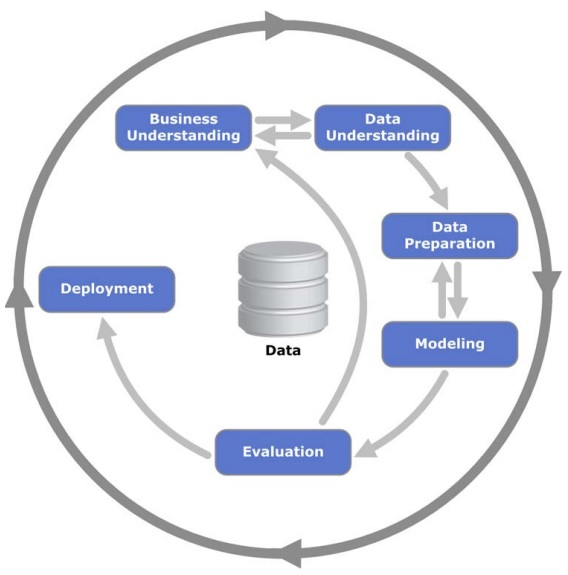
\includegraphics[width=80mm,scale=0.8]{assets/crispdm.jpg}
	}
	\caption{Phases of the CRISP-DM Process Model}
	\label{fig1}
\end{figure}

As atividades que compreendem este artigo serão realizadas conforme as seguintes etapas do CRISP-DM a seguir:

\begin{enumerate}
	\item Compreensão do negócio: o contexto do problema apresentado será analisado com detalhe para uma melhor compreensão da vulnerabilidade feminina.
	\item Compreensão dos dados: os dados do RAIS serão coletados e examinados para identificar problemas de qualidade e verificar se eles são adequados para atender aos objetivos da pesquisa. Além disso, serão identificadas as variáveis que serão utilizadas na análise.
	\item Preparação dos dados: os dados da RAIS serão preparados para análise, o que pode incluir a limpeza de dados, a transformação de variáveis e a seleção de subconjuntos de dados relevantes. 
	\item Modelagem: serão aplicados modelos estatísticos ou de aprendizado de máquina para identificar padrões nos dados da RAIS, bem como relações entre variáveis.
	\item Avaliação: os resultados da modelagem serão avaliados para verificar se eles atendem aos objetivos da pesquisa, isto é, se eles fornecem informações úteis.
	\item Implantação: nesta etapa final, os resultados serão apresentados e as hipóteses confirmadas ou refutadas.     	      	      	      	      	      
\end{enumerate}


\subsection{Compreensão dos dados}

Controlou-se um vetor de fatores individuais (idade e tempo de emprego) e empresariais
(região, tamanho e atividade econômica), que podem afetar o salário. A Tabela \ref{vars} apresenta e
descreve as variáveis explicativas desta tese.

\begin{table}[htbp]
	\caption{Dados analisados}
	\begin{center}
		\begin{tabular}{|c|c|c|}
			\hline
			\textbf{Variável}            & \textbf{Definição}     & \textbf{Exemplo}    \\ 
			\hline 
			\textbf{Remuneração Média} & Com base no ano          & 5000                \\
			\hline
			\textbf{Desligamento}         & Desligamento da empresa  & 0, -1               \\
			\hline 
			\textbf{Região}              & Localização da empresa & MS, DF              \\
			\hline 
			\textbf{Ocupação}           & Descrição do cargo     & Analista de suporte \\
			\hline 
			\textbf{Ano}                  & Período dos dados       & 2018, 2019          \\
			\hline
		\end{tabular}
		\label{vars}
	\end{center}
\end{table}
